 \documentclass[xcolor=dvipsnames, aspectratio=169, 10pt]{beamer}

\usetheme[sectionpage=progressbar,subsectionpage=progressbar]{metropolis}
\usepackage{tikz}
\usetikzlibrary{bayesnet}
\usetikzlibrary{arrows}
\usetikzlibrary{backgrounds}
\usepackage{caption}
\usepackage{animate}
\usepackage{bm}
\usepackage[lined,commentsnumbered]{algorithm2e}
\beamertemplatenavigationsymbolsempty
\usepackage{mathtools}
\usepackage{amsthm}
\usepackage{proof}


\usepackage{tikz}
\usetikzlibrary {automata,positioning}

\definecolor{background}{HTML}{274150}
\definecolor{sbackground}{HTML}{b51823}
\definecolor{main-text}{HTML}{80A07C}
\definecolor{enumercolor}{HTML}{A4CCE0}
\definecolor{progress-bar}{HTML}{E6CBA0}\usecolortheme[named=sbackground]{structure} % define for item color, commented Jan 4,2024

\setbeamertemplate{section in toc}[circle]
\setbeamercolor{section in toc}{bg=sbackground!40, fg=black} % change color section item
 \setbeamerfont{section number projected}{size=\large}
% ENUM
  % \setbeamercolor{item projected}{bg=red!70!black,fg=white}
  \setbeamercolor{frametitle}{fg=sbackground,bg=sbackground!40} % change color bar
  \setbeamercolor{background canvas}{bg=white} % change color frame
  \setbeamercolor{normal text}{fg=black} % change text color
\setbeamercolor{progress bar}{fg=progress-bar!110,bg=progress-bar!50} % change progress bar color
    \setbeamertemplate{enumerate items}[circle]
    \setbeamerfont{itemize item projected}{size=\huge}
        \setbeamerfont{item projected}{size=\large}
% CAPTION
\setbeamertemplate{caption}{\raggedright\insertcaption\par}
% LOGO
\usepackage{textpos} 

\addtobeamertemplate{frametitle}{}{%
	\begin{textblock*}{100mm}(\textwidth,-.9cm)
		% 
\includegraphics[height=.7cm,width=.7cm]{logo.png}
\end{textblock*}}
\usepackage{eso-pic}
\usepackage{pgf}
\titlegraphic{
	% \begin{picture}(0,0)
	% 	\put(420,5){\makebox(0,0)[rt]{
\includegraphics[width=3cm]{logo.png}}}
	% \end{picture}
}
\setbeamertemplate{bibliography item}{\insertbiblabel}
\newcommand{\nologo}{\setbeamertemplate{logo}{}}

\usepackage{commands}
% HEADLINE
%\setbeamertemplate{headline}{}
% FOOTLINE
\setbeamercolor{custom1}{fg=black,bg=mycolor}
\setbeamercolor{custom2}{fg=black, }
\setbeamercolor{custom3}{fg=black,}
\setbeamerfont{footline}{series=\bfseries}%, family=\ttfamily}
\setbeamertemplate{footline}{%
	\leavevmode%

	\begin{beamercolorbox}[wd=1\textwidth, sep=0.4em, right]{custom3}%
		\strut \insertframenumber/\inserttotalframenumber
	\end{beamercolorbox}%
}
% Thank you slide
\makeatletter
\let\beamer@writeslidentry@miniframeson=\beamer@writeslidentry%
\def\beamer@writeslidentry@miniframesoff{%
	\expandafter\beamer@ifempty\expandafter{\beamer@framestartpage}{}% does not happen normally
	{%else
		% removed \addtocontents commands
		\clearpage\beamer@notesactions%
	}
}
\newcommand*{\miniframeson}{\let\beamer@writeslidentry=\beamer@writeslidentry@miniframeson}
\newcommand*{\miniframesoff}{\let\beamer@writeslidentry=\beamer@writeslidentry@miniframesoff}
\makeatother
\usepackage{stmaryrd}
% COMMAND
\newcommand\norm[1]{\left\lVert#1\right\rVert}

% Remove main reference numbering
\setbeamertemplate{frametitle continuation}{}

%% TITLE PAGE 
\title[]{Session Types}

% DOCUMENT
\begin{document}
\date{}
\captionsetup[figure]{labelformat=empty, font={footnotesize,it}}
\begin{frame}[noframenumbering,plain]
	\titlepage
\end{frame}

\begin{frame}
	\frametitle{Outline}
	\tableofcontents
\end{frame}

\section{Multiparty Session Types}

\begin{frame}{Syntax}
  \begin{figure}[ht]
    $$\begin{array}{lclr}
        T & ::= & S & \text{(session type)} \\
          & |   & D & \text{(data type)}
      \end{array}$$

    \begin{center}
      \begin{minipage}{0.45\textwidth}
        $$\begin{array}{lclr}
            S & ::= & \texttt{end} & \text{(termination)}    \\
              & |   & L.S          & \text{(sequence)}       \\
              & |   & \mu\alpha.S  & \text{(recursion)}      \\
              & |   & \alpha       & \text{(type variable)}  \\
              & |   & (S+S)        & \text{(nondeterminism)} \\
          \end{array}$$
      \end{minipage}
      \hfill
      \begin{minipage}{0.53\textwidth}
        $$\begin{array}{lclr}
            L    & ::= & L | L                                                         & \text{(asynchrony)}   \\
                 & |   & p\rightarrow q(D)                                             & \text{(send-receive)} \\
                 & |   & \texttt{skip}                                                 & \text{(skip)}         \\
            p,q  & \in & \ZZ\cup\{\infty\}, p\ne q, pq\ge 0                            & \text{(index)}        \\
            D    & ::= & \ell | \texttt{bool} | \texttt{int} | \texttt{string} |\ldots &                       \\
            \ell & \in & \L                                                            & \text{(label)}        \\
          \end{array}$$
      \end{minipage}
    \end{center}
    % \caption{The syntax of extended multiparty session type}
    \label{syntax}
  \end{figure}
\end{frame}

\begin{frame}{Operational Semantics}
  $$\begin{array}{lr}
      L.S \xrightarrow{\makebox[1cm][c]{L}} S
                                                      & \text{(sequence)}       \\
      \mu\alpha.S
      \xrightarrow{\makebox[1cm][c]{\texttt{skip}}} \alpha
      \xrightarrow{\makebox[1cm][c]{\texttt{skip}}} S & \text{(recursion)}      \\

      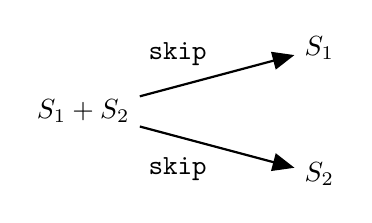
\begin{tikzpicture}[baseline={(current bounding box.center)}, ->, thick]
        \node (src) at (0,0) {\( S_1 + S_2 \)};
        \node (tgt1) at (3,0.8) {\( S_1 \)};
        \node (tgt2) at (3,-0.8) {\( S_2 \)};

        \draw[->] (src) -- node[above left] {\texttt{skip}} (tgt1);
        \draw[->] (src) -- node[below left] {\texttt{skip}} (tgt2);
      \end{tikzpicture}

                                                      & \text{(nondeterminism)} \\
    \end{array}$$
  \textbf{Note:}
  \begin{itemize}
    \item A type $S$ generates a directed graph (NFA) $\text{gr}(S)$ called a semantic graph, with an initial node and the terminal node $\texttt{end}$. We can rename the nodes for convenience.
    \item From the graph, we can show commutativity and distributivity of nondeterminism. Hence we can just write $S_1+S_2+S_3$ instead of $(S_1+S_2)+S_3$.
    \item Conversely, for each directed graph whose edges are defined by the production rules for $L$ (can have multiple terminal nodes), we have a type.
  \end{itemize}



\end{frame}

\begin{frame}{Subtype}
  We want to encode in our type system
  \begin{itemize}
    \item Determinism is allowed in a nondeterministic context
          $$S_1\preceq S_1+S_2.$$
    \item Waiting for more actions to be asynchronously executed is allowed
          $$L_1|L_2 \preceq L_1.$$
  \end{itemize}

  The latter can be expressed as a relation between two \textit{edges}.
\end{frame}

\begin{frame}{Trace and Path}
  A path is a sequence $S_1\xrightarrow{L_1}S_2\xrightarrow{L_2}\cdots\xrightarrow{L_n}\texttt{end}$. Given this path, we have a trace $t=L_1.L_2 \ldots L_n$. The length of $t$ is $|t|=n$.

  A trace $t=L_1.L_2 \ldots L_n$ is equivalent to the path from $t$ removing a \texttt{skip}
  $$L_1.L_2 \ldots L_n \equiv L_1\ldots L_{j-1}.L_j\ldots L_n \text{ if } L_j = \texttt{skip}.$$

  Let $t=L_1.L_2 \ldots L_n$ and $t'=L'_1.L'_2 \ldots L'_n$. Define $t\preceq t'$ if $L_i\preceq L'_i$ for all $i\in\{1,\ldots,n\}$.

  Let $t_1$ and $t_2$ be two traces. Then $t_1\preceq t_2$ if there exist $t'_1$ and $t'_2$ of the same length such that $t_1 \equiv t'_1$, $t_2 \equiv t'_2$ and $t'_1\preceq t'_2$.
\end{frame}

\begin{frame}{Subtype}
  Hence we can define subtype relation based on generated graphs.

  Let $\text{tr}(S)$ the set of traces of the graph generated by $S$.

  We define $S_1\preceq S_2$ if for any $t_1\in\text{tr}(S_1)$, there exists $t_2\in\text{tr}(S_2)$ such that $t_1\preceq t_2$.

  But the best thing we should do is to derive equational reasoning on types.

  \begin{itemize}
    \item For each type $S$, there exists a corresponding \textit{regular expression}.
    \item There have been proof theories on regular expressions (Kleen algebra) and right-linear grammar \footnote{Das, Anupam, and Abhishek De. "A proof theory of right-linear ($\omega$-) grammars via cyclic proofs." Proceedings of the 39th Annual ACM/IEEE Symposium on Logic in Computer Science. 2024.}
  \end{itemize}
\end{frame}

\begin{frame}{Projection}
  \begin{center}
    \begin{minipage}{0.48\textwidth}
      $$\begin{array}{rlr}
          p\rightarrow q \downharpoonright_p & =

          \begin{cases}
            0\rightarrow \infty, & \text{ if } q=0   \\
            0\rightarrow -q,     & \text{ if } q < 0 \\
            \varnothing,         & \text{ otherwise} \\
          \end{cases}
        \end{array}$$
    \end{minipage}
    \hfill
    \begin{minipage}{0.48\textwidth}
      $$\begin{array}{rlr}
          q\rightarrow p \downharpoonright_p & =
          \begin{cases}
            \infty\rightarrow 0, & \text{ if } q=0   \\
            -q\rightarrow 0,     & \text{ if } q < 0 \\
            \varnothing,         & \text{ otherwise} \\
          \end{cases}
        \end{array}$$
    \end{minipage}
  \end{center}

  $$\begin{array}{rlr}
      L_1|L_2 \downharpoonright_p           & =
      L_1\downharpoonright_p | L_2 \downharpoonright_p                                                   \\
      \texttt{skip}\downharpoonright_p      & = \texttt{skip}                                            \\

      p\rightarrow q (D)\downharpoonright_p & =
      \begin{cases}
        p\rightarrow q\downharpoonright_p (D), \text{ if } p\rightarrow q\downharpoonright_p\ne\varnothing \\
        \texttt{skip}, \text{ otherwise}
      \end{cases} \\
    \end{array}$$

  From $\text{gr}(S)$, we replace each edge by its projection. The type derived from this graph is the projected type $S\downharpoonright_p$.

  \textbf{Proposition:} If $S_1\preceq S_2$, then $S_1\downharpoonright_p \preceq S_2\downharpoonright_p,\forall p \in \NN^{-}$.
\end{frame}


\section{Typed Open Automata}
\begin{frame}{Typed Open Automata}
  A typed open automaton is a tuple $A=\langle S, s_0, E, V, \phi_0, T\rangle$, where
  \begin{itemize}
    \item $S$ is the set of states
    \item $s_0\in S$ is the initial state
    \item $E\subset S$ is the set of terminal states
    \item $V$ is the set of variables
    \item $\psi_0: V\to\P$ is the initial assignment
    \item $T$ is the set of transitions. Each $t\in T$ has the form $\dfrac{\beta_{j}^{j\in J}, g, \psi}{s\xrightarrow{\alpha}s'}$, where
          \begin{itemize}
            \item [$\circ$]$s,s'\in S$ and $\alpha$ is an emitted action.
            \item [$\circ$] each $\beta_{j}$ has the form $p\to q(m : D)$ or $p\to q(\ell)$ such that $p,q\in \ZZ\cup\infty$, $p\ne q$, $pq\ge0$ and $\ell\in\L$.
            \item [$\circ$] $g$ is a predicate over $V$
            \item [$\circ$] $\psi: V\to \E_V$ is a reassignment
          \end{itemize}
  \end{itemize}
  We can ignore the emitted action and write $s\xrightarrow{\beta_{j}^{j\in J}, g, \psi}s'$. A pair $(s, \phi)$, where $s\in S$ and $\phi:V\to\P$ is called a configuration of the automaton.
\end{frame}

\begin{frame}{Example}
  Consider a producer-consumer communication through a size-2 circular buffer. This is modeled as an automaton $A$.

  \begin{figure}[ht]
    \centering
    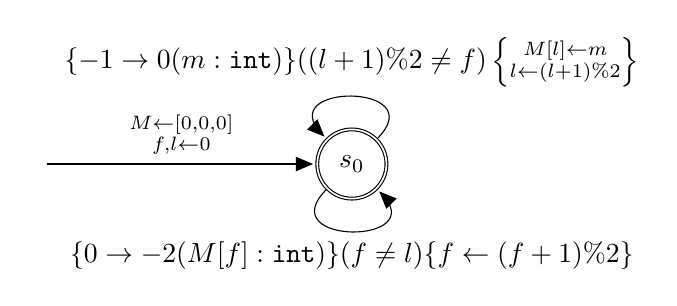
\begin{tikzpicture}[shorten >=1pt,node distance=2cm,on grid,auto]

      \node[]               (init_assign){};
      \node[state, accepting] (s_0) [right=4cm of init_assign] {$s_0$};

      \path[->]
      (init_assign) edge node {$\substack{
              M     \leftarrow [0,0,0] \\
              f, l  \leftarrow 0
            }$} (s_0)
      (s_0) edge[loop, in=135, out=45, looseness=4] node[anchor=south] {$\{-1\to0(m:\texttt{int})\}((l+1)\%2\ne f)\left\{\substack{M[l]\leftarrow m\\l\leftarrow (l+1)\%2}\right\}$} (s_0)
      (s_0) edge[loop, in=-45, out=-135, looseness=4] node[anchor=north] {$\{0\to -2(M[f]:\texttt{int})\}(f\ne l)\{f\leftarrow (f+1)\%2\}$} (s_0)
      ;
    \end{tikzpicture}
  \end{figure}
\end{frame}

\begin{frame}{Type Generated by an OA}
  Consider $A=\langle S, s_0, E, V, \phi_0, T\rangle$.
  \begin{itemize}
    \item $\llbracket p\to q(m : D)\rrbracket = p\to q(D)$
    \item $\llbracket p\to q(\ell)\rrbracket = p\to q(\ell)$
    \item $\llbracket \beta_1,\ldots,\beta_n \rrbracket = \llbracket \beta_1 \rrbracket | \ldots | \llbracket \beta_n \rrbracket$
  \end{itemize}
\end{frame}

\begin{frame}{Weak type}
  The weak type $W_A$ generated by $A$ is derive from the graph, called the weak type graph, such that
  \begin{itemize}
    \item The set of nodes is $S$, the initial node is $s_0$, the set of terminal nodes is $E$
    \item Each transition $s\xrightarrow{\beta_{j}^{j\in J}, g, \psi}s'$ has a corresponding edge $s\xrightarrow{\llbracket \beta_{j}^{j\in J} \rrbracket}s'$
  \end{itemize}

  \textbf{Example:} The weak type graph for producer-consumer. Let $U=-1\to0(\texttt{int})$ and $V=0\to -2(\texttt{int})$. The type is $W_A=\mu\alpha.(\texttt{end}+U+V).\alpha$

  \begin{figure}[ht]
    \centering
    \begin{tikzpicture}[shorten >=1pt,node distance=2cm,on grid,auto]

      \node[state, accepting] (s_0) [below=2cm of init_assign] {$s_0$};

      \path[->]
      (s_0) edge[loop, in=135, out=45, looseness=4] node[anchor=south] {$-1\to0(\texttt{int})$} (s_0)
      (s_0) edge[loop, in=-45, out=-135, looseness=4] node[anchor=north] {$0\to -2(\texttt{int})$} (s_0)
      ;
    \end{tikzpicture}
    \caption{The DFA generated by the weak type of $A$}
  \end{figure}
\end{frame}

\begin{frame}{Strong type}
  The strong type graph $G_S$ has nodes as \textit{configurations}. The initial node is $(s_0,\phi_0)$. Terminal nodes are $(s, \psi)$ where $s\in E$.

  Each $(s,\phi)\xrightarrow{\beta_{j}^{j\in J}, g, \psi}(s',\phi')$ corresponds to an edge $(s,\phi)\xrightarrow{\llbracket\beta_{j}^{j\in J}\rrbracket}(s',\phi')$.

  The graph $G_S$ derives the strong type $S_A$.

  We should be able to show that $S_A\preceq W_A$.

  \textbf{Example:} The strong type graph for producer-consumer.

\end{frame}

\begin{frame}{Strong type}
  \begin{figure}
    \centering
    \resizebox{0.5\textwidth}{!}{
      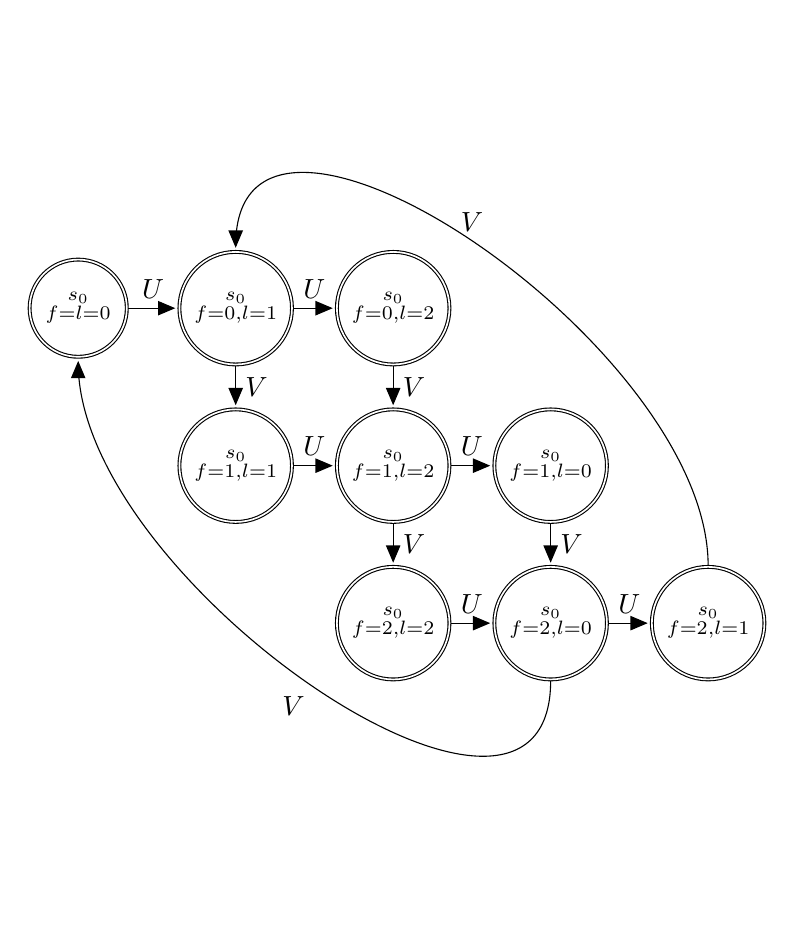
\begin{tikzpicture}[shorten >=1pt,node distance=2cm,on grid,auto]

        \node[state, accepting] (w_00) {$\substack{s_0\\ f=l=0}$};
        \node[state, accepting] (w_01) [right=2cm of w_00] {$\substack{s_0\\ f=0,l=1}$};
        \node[state, accepting] (w_02) [right=2cm of w_01] {$\substack{s_0\\ f=0,l=2}$};

        \node[state, accepting] (w_11) [below=2cm of w_01] {$\substack{s_0\\ f=1,l=1}$};
        \node[state, accepting] (w_12) [below=2cm of w_02] {$\substack{s_0\\ f=1,l=2}$};

        \node[state, accepting] (w_10) [right=2cm of w_12] {$\substack{s_0\\ f=1,l=0}$};

        \node[state, accepting] (w_20) [below=2cm of w_10] {$\substack{s_0\\ f=2,l=0}$};
        \node[state, accepting] (w_22) [below=2cm of w_12] {$\substack{s_0\\ f=2,l=2}$};

        \node[state, accepting] (w_21) [right=2cm of w_20] {$\substack{s_0\\ f=2,l=1}$};


        \path[->]
        (w_00) edge[] node[anchor=south] {$U$} (w_01)
        (w_01) edge[] node[anchor=south] {$U$} (w_02)

        (w_01) edge[] node {$V$} (w_11)
        (w_02) edge[] node {$V$} (w_12)

        (w_11) edge[] node {$U$} (w_12)

        (w_12) edge node {$U$} (w_10)
        (w_12) edge node {$V$} (w_22)
        (w_22) edge node {$U$} (w_20)

        (w_10) edge node {$V$} (w_20)
        (w_20) edge node {$U$} (w_21)

        (w_20) edge[out=-90, in=-90] node {$V$} (w_00)
        (w_21) edge[out=90, in=90] node[anchor=south] {$V$} (w_01)
        ;
      \end{tikzpicture}}
  \end{figure}
\end{frame}

\begin{frame}{Strong type}

  However, the strong type does not always exist i.e. strong type graph generation does not always halt.

  \textbf{Example:}  Consider a key-generating protocol, where the server request generating a secret key for the client to use later. The number of key consumptions cannot exceed the number of key generation requests. This is modeled as an automaton $B$.

  \begin{figure}[ht]
    \centering
    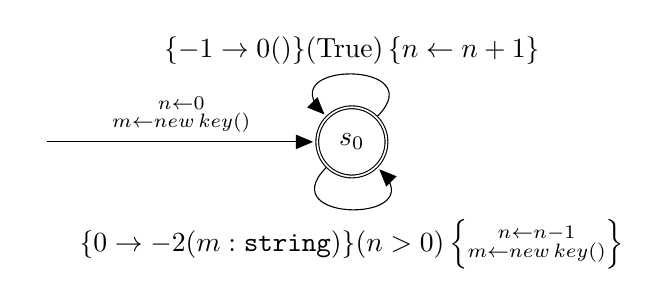
\begin{tikzpicture}[shorten >=1pt,node distance=2cm,on grid,auto]

      \node[]               (init_assign){};
      \node[state, accepting] (s_0) [right=4cm of init_assign] {$s_0$};

      \path[->]
      (init_assign) edge node {$\substack{
              n\leftarrow 0\\
              m\leftarrow new \, key()
            }$} (s_0)
      (s_0) edge[loop, in=135, out=45, looseness=4] node[anchor=south] {$\{-1\to0()\}(\text{True})\left\{n\leftarrow n+1\right\}$} (s_0)
      (s_0) edge[loop, in=-45, out=-135, looseness=4] node[anchor=north] {$\{0\to -2(m:\texttt{string})\}(n>0)\left\{\substack{n\leftarrow n-1\\  m\leftarrow new \, key()}\right\}$} (s_0)
      ;
    \end{tikzpicture}
  \end{figure}
\end{frame}

\begin{frame}{Relaxed type}
  A relaxed type graph $G_R$ has nodes of the form $(s,P)$, where $P$ is a predicate over $V$. \textit{The} initial node is $(s_0,P_0)$ such that $\phi_0\vdash P_0$. Terminal nodes are $(s, P)$ where $s\in E$.

  Each $(s,\phi)\xrightarrow{\beta_{j}^{j\in J}, g, \psi}(s',\phi')$ corresponds to an \textit{edges} $(s,P)\xrightarrow{\llbracket\beta_{j}^{j\in J}\rrbracket}(s',P')$ such that $\phi\vdash P$ and $\phi'\vdash P'$

  The graph $G_R$ derives the strong type $R_A$.

  We should be able to show that $S_A\preceq R_A\preceq W_A$.
\end{frame}

\begin{frame}{Relaxed type}
  \textbf{Example:} Let $X=-1\to0(\texttt{void})$ and $Y=0\to -2(\texttt{string})$. We have relaxed type graph for key-generating protocol which derives
  $$R_B=\mu\alpha_0.X.\mu\alpha_1.(X.\alpha_1+ Y.\alpha_1 + Y.\alpha_0).$$
  \begin{figure}[ht]
    \centering
    \begin{tikzpicture}[shorten >=1pt,node distance=2cm,on grid,auto]

      \node[state, accepting] (s_0) [below=2cm of init_assign] {$s_0, n=0$};

      \node[state, accepting] (s_1) [right=3cm of s_0] {$s_0, n>0$};

      \path[->]
      (s_0) edge[out=45, in=135] node[anchor=south] {$X$} (s_1)
      (s_1) edge[loop, out=45, in=-45, looseness=4] node[] {$X,Y$} (s_1)
      (s_1) edge[out=-135, in=-45] node[] {$Y$} (s_0)
      ;
    \end{tikzpicture}
  \end{figure}
\end{frame}

\begin{frame}{Relaxed type}
  \textbf{Example:} Another relaxed type graph for key-generating protocol. It derives $R'_B$.
  \begin{figure}[ht]
    \centering
    \begin{tikzpicture}[shorten >=1pt,node distance=2cm,on grid,auto]

      \node[state, accepting] (s_0) [below=2cm of init_assign] {$s_0, n=0$};
      \node[state, accepting] (s_1) [right=3cm of s_0] {$s_0, n=1$};
      \node[state, accepting] (s_2) [right=3cm of s_1] {$s_0, n>1$};

      \path[->]
      (s_0) edge[out=45, in=135] node[anchor=south] {$X$} (s_1)
      (s_1) edge[out=-135, in=-45] node[] {$Y$} (s_0)

      (s_1) edge[out=45, in=135] node[anchor=south] {$X$} (s_2)
      (s_2) edge[out=-135, in=-45] node[] {$Y$} (s_1)

      (s_2) edge[loop, out=45, in=-45, looseness=4] node[] {$X,Y$} (s_2)
      ;
    \end{tikzpicture}
  \end{figure}
  Note that $R'_B\prec R_B$ (strictly) but $R'_B\downharpoonright_{-1}\equiv R_B \downharpoonright_{-1}$.
\end{frame}


\begin{frame}{Directions}
  Let $\S(A)$ be the set of types generated by $A$ (strongly, weakly and relaxedly). We attempt to prove or disprove that
  \begin{itemize}
    \item $\S(A)$ is totally ordered. In particular, if $S_1$ and $S_2$ are generated by an automaton $A$, then $S_1\preceq S_2$ if and only if the number of nodes $\text{gr}(S_1)$ is greater than or equal to the number of nodes in $\text{gr}(S_2)$.
    \item If there exist $S_1,S_2\in\S(A)$ such that $S_1\not\equiv S_2$ and $S_1\downharpoonright_p \equiv S_2\downharpoonright_p$. Then $S\downharpoonright_p\equiv S_1\downharpoonright_p$, for every $S\in \S(A)$.
  \end{itemize}
  \textbf{Note:} If the latter is correct, we may be sure about the type of a child without knowing the strong type of the parent.
\end{frame}

\begin{frame}{Composition}
  Consider an automaton
  $$A=\llangle S_A, s_{0A}, E_A, V_A, \psi_{0A}, T_A\rrangle \text{ and } B=\llangle S_B, s_{0B}, E_B, V_B, \psi_{0B}, T_B\rrangle.$$

  An automaton $B$ can be safely composed to the child indexed by $p$ of the automaton $A$ if $\inf \S(B) \preceq \inf \{S\downharpoonright_p | S\in \S(A)\}$.

  Reindex children of $A$ and $B$ if there is any conflict.
\end{frame}

\begin{frame}{Composition}
  The composition of $B$ into the internal component indexed by $p<0$ of $A$ yields an open automaton $A[B/p]:=C=\llangle S_C, s_{0C}, E_C, V_C, \psi_{0C}\rrangle$, such that
  \begin{itemize}
    \item $S_C = S_A\times S_B$
    \item $s_{0C} = (s_{0A}, s_{0B})$
    \item $E_C = E_A\times E_B$
    \item $V_C = V_A\uplus V_B$
    \item $\psi_C = \psi_A\uplus \psi_B$
    \item $T_C = \ldots$
  \end{itemize}
\end{frame}

\begin{frame}
  \begin{align*}
    T_C & = \left\{\dfrac{\beta_{j''}^{j''\in J''}, g\wedge g', \psi\uplus\psi'}{(s,s')\xrightarrow{\alpha} (t,t')}\Bigg|\dfrac{\beta_{j}^{j\in J}, g, \psi}{s\xrightarrow{\alpha} t}\in T_A\wedge \dfrac{\beta_{j'}^{j'\in J'}, g', \psi'}{s'\xrightarrow{\alpha'} t'}\in T_B\wedge \llbracket \beta_{j'}^{j'\in J'}\rrbracket \preceq \llbracket \beta_{j}^{j\in J}\rrbracket\downharpoonright_p \right\}                   \\
        & \bigcup \left\{\dfrac{\beta_{j}^{j\in J}, g, \psi}{(s,s')\xrightarrow{\alpha} (t,t')}\Bigg|s',t'\in S_B\wedge\dfrac{\beta_{j}^{j\in J}, g, \psi}{s\xrightarrow{\alpha} t}\in T_A \wedge \left(\not\exists\dfrac{\beta_{j'}^{j'\in J'}, g', \psi'}{s'\xrightarrow{\alpha'} t'}\in T_B, \llbracket \beta_{j'}^{j'\in J'}\rrbracket \preceq \llbracket \beta_{j}^{j\in J}\rrbracket\downharpoonright_p\right) \right\} \\
        & \bigcup \left\{\ldots\Bigg|\dfrac{\beta_{j'}^{j'\in J'}, g', \psi'}{s'\xrightarrow{\alpha'} t'}\in T_B\wedge \left(\not\exists \dfrac{\beta_{j}^{j\in J}, g, \psi}{s\xrightarrow{\alpha} t}\in T_A, \llbracket \beta_{j'}^{j'\in J'}\rrbracket \preceq \llbracket \beta_{j}^{j\in J}\rrbracket\downharpoonright_p\right) \right\}
  \end{align*}

  We have to work more on the last set. Generally speaking, all other communications in $B$ become internal communication in $A[B/p]$.
\end{frame}

\begin{frame}{Plans}
  \begin{itemize}
    \item That $\inf \S(A[B/p]) \prec \inf \S(A)$ is not straightforward
  \end{itemize}
\end{frame}



\begin{frame}
	\begin{center}
		\Huge\textbf{Thank you for listening !}
	\end{center}
\end{frame}
% \printbsibliography
\end{document}